\section{Derivation}
It is possible to further optimize the filter using the look-ahead technique, which simply consists in unrolling a recursive relation to obtain another equivalent one that depends explicitly on instants further back in time. The aim is to introduce a larger delay in the feedback loop so as to reduce $T_{\infty}$, paving the way for universal techniques such as retiming.\\
Considering \autoref{eqn:iir}, notice that $w[n-1]$ appears in the expressions for $w[n]$ and $y[n]$.
\begin{align}
	w[n-1] = x[n-1] - a_1 w[n-2]
	\label{eqn:w-lookahead}
\end{align}
Substituting \autoref{eqn:w-lookahead} back into both the equations that define direct form II (\autoref{eqn:iir}):
\begin{align}
	\begin{cases}
		w[n] &= x[n] - a_1 x[n-1] + a_1^2 w[n-2] 		\\
		y[n] &= b_1 x[n-1] + b_0 w[n] - a_1 b_1 w[n-2]
	\end{cases}
	\label{eqn:iir-lookahead-bad}
\end{align}

\autoref{eqn:iir-lookahead-bad} shows the result obtained by performing the same substitution in the output equation as well. It is clear that this is not convenient because the number of operators required in the feedforward part would be increased unnecessarily. In fact, the look-ahead technique is very useful in tackling loops that cannot be sped up using universal techniques either because there are too few registers involved or they might have an unacceptably large $T_{\infty}$. It is not really well suited for purely feedforward structures within the DFG, where standard pipelining can effectively cut critical paths. In conclusion, the solution is to use the new expression for $w[n]$ (which includes a feedback) while retaining the unmodified $y[n]$. In this way, $b_1 x[n-1]$ does not appear in the equation for $y[n]$, saving one multiplier and one adder, while still allowing a complete optimization that, as will be discussed, brings the critical delay down to $T_{CP}=1 \times T_\text{mul}$.
\\
The \textbf{final set of equations} used in the look-ahead architecture is the following:
\begin{align}
	\begin{cases}
		w[n] &= x[n] - a_1 x[n-1] + a_1^2 w[n-2] 		\\
		y[n] &= b_0 w[n] + b_1 w[n-1]
	\end{cases}
	\label{eqn:iir-lookahead}
\end{align}
Its implementation and optimizations are explored in the following sections.

\subsection{Retiming and pipelining}
The preliminary result of a direct mapping of these equations into a DFG is in \autoref{fig:fast_dfg_inter}. It is clear that pipeline registers can be placed on feedforward cutsets in order to break critical paths. Since the feedback loop sets a lower bound on $T_{cp}$, retiming will be applied first in order to leverage the possibilities opened by the look-ahead transformation, and only then the correct distribution of pipeline stages will be determined accordingly.

\paragraph{Retiming} As for the feedback loop, it is clear that look-ahead has changed $T_{\infty}$ that has now decreased to $\frac{T_m+T_a}{2}$. Moreover, the introduction of a second register enables the use of retiming to bring the critical path closer the its lower bound (loop bound). By moving the pink register in the position indicated by the dashed arrow, thus separating the multiplier from the adder, $T_{CP}$ is reduced to $T_m$ (assuming $T_m > T_a$). Another slight optimization consists in replacing the two orange registers by a single one positioned at the output of the adder, as can be seen in figure \autoref{fig:fast_dfg_final}.

\paragraph{Pipeline stages} The loop contains a critical path equal to a single multiplier delay, therefore the correct number and placement of pipeline register is to be determined so as to remove any feedforward path with a delay larger than $T_m$. It follows that there must be a delay element on every edge joining an adder and a multiplier ($T_m + T_a > T_m$). The stages indicated with the blue and brown dashed lines in figure \autoref{fig:fast_dfg_inter} serve exactly this purpose. On the other hand, the yellow line corresponds to a pipeline stage separating two adders: this is actually useful only if $2T_a>T_m$. According to timing reports collected during the synthesis of the standard architecture, DesignWare can provide operators with delays as low as $T_m = 0.82 \,\textrm{ns}$ and $T_a=0.32\,\textrm{ns}$ when constrained for maximum speed. These numbers suggest that the path formed by \texttt{A1} and \texttt{A2} without the interposed yellow register is not the critical one since the multiplier has still a slightly larger delay ($T_m=0.82 > 2T_a =0.64$). However, the implementation of fast operators might involve larger structures in terms of area (complexity). In short, there is a trade off and the optimal solution depends on the actual parameters of the available library cells and the specific design goals. In order to assess the impact of adding the yellow pipeline stage, the two cases have been synthesized separately. Since the aim is to discover the impact on performance (speed), these synthesis are run with a constraint on $T_{clk}$ set to zero.

\begin{table}[h]
	\centering
\begin{tabular}{|l|l|l|}
	\hline
\textbf{Parameter}	&  \textbf{2 pipeline stages} & \textbf{3 pipeline stages} \\\hhline{|=|=|=|}
Minimum clock period & 1.05 ns & 1.02 ns\\\hline
Adder Area & 51.9 (Buf/Inv 6.9) & 48.4 (Buf/Inv 6.9)\\
Combinational Area & 1389 & 1437\\
Buf/Inv Area& 163 & 168\\
Noncombinational Area& 466 & 505\\
Overall area & 1856 & 1942\\
\hline
Dynamic power ($T_{ck}=4.08\,\textrm{ns}$) & 252 $\mu$W & 260 $\mu$W \\
\hline
\end{tabular}
\caption{Comparison showing the impact of the yellow register. Synthesis is performed for maximum speed for all parameters except for dynamic power, which has been derived at fixed $f_{clk}$ for a fair assessment}
\label{tab:comparison}
\end{table}

\autoref{tab:comparison} shows that the compiler finds a slightly faster solution (3\%) when synthesizing the design with the additional pipeline stage. This is not due to a different critical path, because both timing reports list the path through a multiplier. It is more likely a consequence of the heuristic nature of the algorithm used to search the design space, which targets a global optimization with a complex cost function that accounts for several factors beside speed.\\
As for the area used up by adders, it becomes 7\% larger if the yellow stage is removed, with buffers taking up more space. In fact, breaking the path \texttt{A1-A2} could also translate into a more relaxed constraint on the delay of each one of them, perhaps attainable with simpler and more compact architectures. However, the area used up by the register itself largely outweighs this reduction (see \textit{Noncombinatinal area}), resulting in a larger overall area. Dynamic power consumption is 4\% higher if the pipeline stage is added.
\\In conclusion, this comparison shows that an higher speed is obtained when all operators are isolated by pipeline registers, but this results in a slight increase in area and power dissipation. If the aim is maximum performance the alternative with $T_{min}\approx 1.02 \,\textrm{ns}$ is the best choice, whereas a strategy that prioritizes area or power would lead to the opposite conclusion.
The final DFG that corresponds to the actual VHDL implementation is in figure \ref{fig:fast_dfg_final}.
\paragraph{A formal approach to retiming} Retiming can be easily done by inspection in this particular case, as shown in \autoref{fig:fast_dfg_inter}. However, for larger designs this task cannot be handled without a more formal and algorithmic approach. The problem can be cast as a system of inequalities expressing the feasibility constraint for retiming, which states that the final number of delays on each edge must be nonnegative. Moreover, there has to be at least one register on paths joining operators whose combined delay is larger than the critical path. The introduction of pipeline stages can be equivalently thought of as inserting a number of input registers and the performing retiming to transfer them to the desired cutsets. In this case this is convenient because both problems can be addressed using this formal approach. The system of inequalities is the following
\begin{align*}
&r(1) + \Delta \geq 0\\
&r(2)+\Delta \geq 0\\
&r(2)-r(1)+1\geq 1\\
&r(3)-r(2)\geq \epsilon\\
&r(3)-r(4) \geq 1\\
&r(4)-r(3)+2 \geq 1\\
&r(5)-r(3)\geq 1\\
&r(6)-r(3)+1\geq 1\\
&r(7)-r(5)\geq 1\\
&r(7)-r(6)\geq 1
\end{align*}
Where $\epsilon$ can be set to $1$ if a register should be in between operators $2$ and $3$ or to $0$ otherwise. $\Delta$ is the (maximum) number of pipeline stages (input registers) to be added.
A solution can be found by building the so-called \textit{constraint graph}, where for each inequality $r_i-r_j < c$  a directed edge is drawn from $j$ to $i$ with a weight equal to $c$. An additional virtual node is connected to all the other nodes by edges of zero length. Finally, an all-point shortest path algorithm is executed on this graph and the result $r_i$ can be found as the shortest path from the virtual node to node $i$.
\begin{figure}
	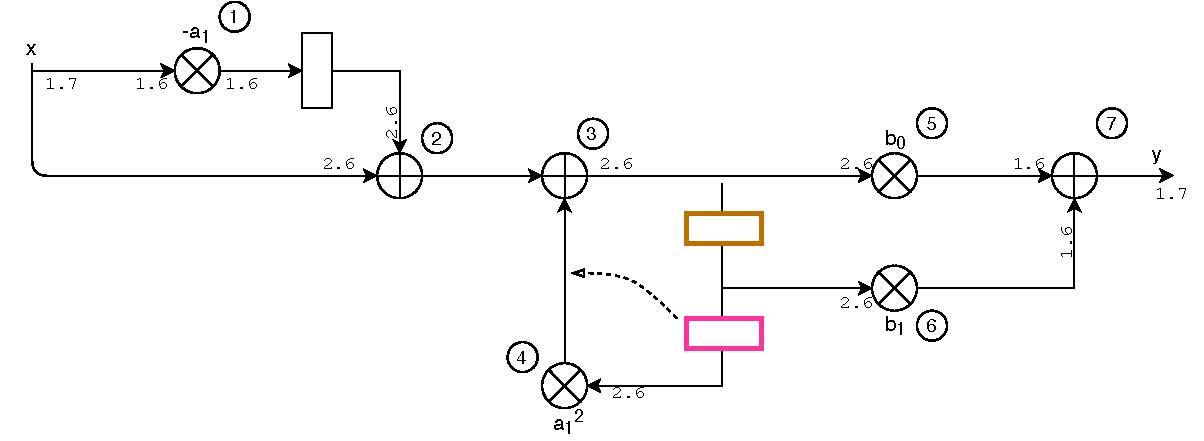
\includegraphics[width=\textwidth]{./chapter2/images/fastdfg_inter_index.pdf}
	\caption{Numbering of operators for the retiming algorithm (system on inequalities)}
\end{figure}
This algorithm has been implemented in the script \texttt{retiming\_algorithm.m} which for this instance returns ($\Delta=3, \,\epsilon=1$):
\begin{equation*}
r = {[}-3, -3, -2, -3, -1, -1, 0{]}
\end{equation*}
which is equivalent to the solution found by inspection (\autoref{fig:fast_dfg_final}).
\subsection{Accuracy}
This new computational structure has also been modeled with a C program in order to perform fast design analyses such as finding of the minimum number of fractional bits that provide the specified accuracy. Although in this case the total harmonic distortion has different values than those found previously, the simulation points towards the same conclusion that a minimum number of $n=7$ bits is necessary.
\subsection{Parallelism}
Similarly to the first architecture, the sequence $w[n]$ can take on values slightly greater than one in magnitude, for example when the input signal is constant and equal to an extremum of the representable range ($2^{7}-1$ or $-2^{7}$). In order to avoid overflow, two integer bits are allocated wherever the intermediate variable $w$ is processed. Slight savings in area can be achieved by allocating only one integer bit for the final adder, since the output of the feedfoward multipliers ($b_0$, $b_1$) and the output variable $y$ are necessarily lower than one in magnitude. The first multiplier ($-a_1$) can also operate on a resized version of $x$ with only 6 fractional bits (as determined in the previous section) and 1 integer bit. In figure \autopageref{fig:fast_dfg_inter} the final parallelism is annotated on every signal. All operators are assumed to operate with the same bitwidth for both the input operands and for the output.  A different labeling on opposite sides of the same line implies that a resizing occurs in between and the same numerical value is represented in different formats by means of sign extension when more integer bits are added, truncation when the number of fractional bit is reduced, removal of the leftmost bits when the value is expected to be small enough to allow the allocation of less integer bits without running into overflow.
\begin{figure}
	\makebox[\textwidth][c]{
	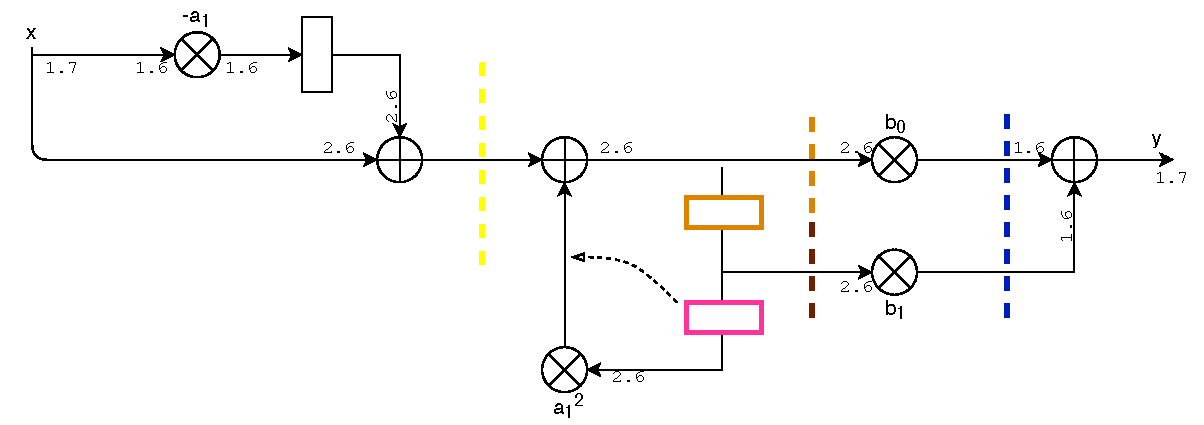
\includegraphics[width=1.2\textwidth]{./chapter3/images/fastdfg_inter.pdf}}
	\caption{Initial DFG with annotated parallelism. Dashed vertical lines indicate cutsets where pipeline stages will be inserted. The pink register
		can be moved to the position indicated by the arrow by means of retiming}
	\label{fig:fast_dfg_inter}
\end{figure}

\begin{figure}
	\makebox[\textwidth][c]{
	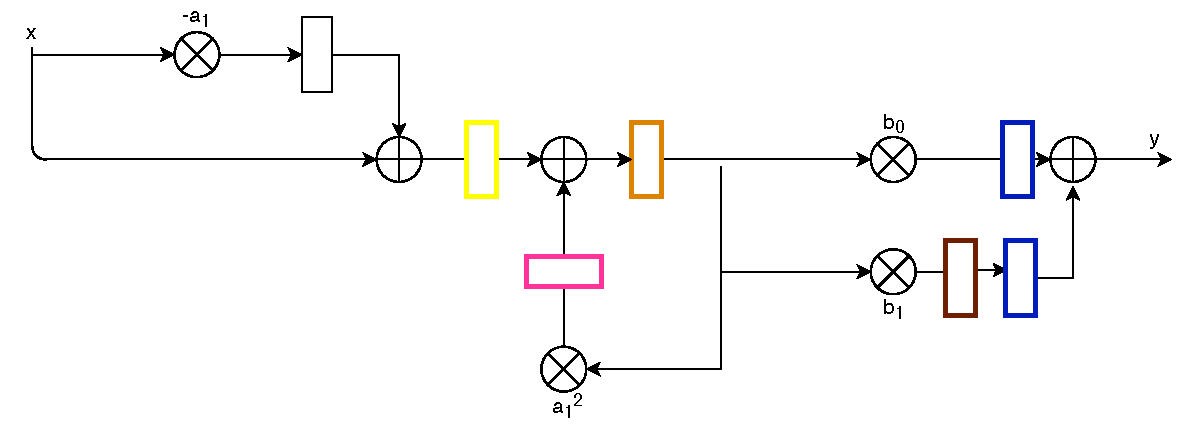
\includegraphics[width=1.2\textwidth]{./chapter3/images/fastdfg_final.pdf}}
	\caption{Final DFG. Colors identify registers corresponding to the DFG in figure \autoref{fig:fast_dfg_inter}}
	\label{fig:fast_dfg_final}
\end{figure}

\section{Control Unit}
The addition of pipeline stages increases dramatically the number of possible states in our FSM, making it impractical to describe the control unit by enumerating all of them. We resorted to a structural description consisting of a delay line where a number of flip-flops are connected in cascade. The delay line contains two flip flops plus one additional flip flop for each pipeline stage, which amounts to a total of five delay units. One additional register samples the reset signal and controls \texttt{clear\_w\_regs}, a signal that causes the unit to enter the reset state for a single clock cycle, where both the datapath registers and the delay line are cleared. The latch enable signal is found at the output of the first flip flop, whereas \texttt{en\_regs} corresponds to the \texttt{Q} output of the second flip-flop, which controls the registers in the feedback path (brown and pink) enabling them when a new data is available in the yellow pipeline register. Finally, VOUT corresponds to the end of the delay line.
